\documentclass{standalone}
\usepackage{tikz}

\begin{document}
    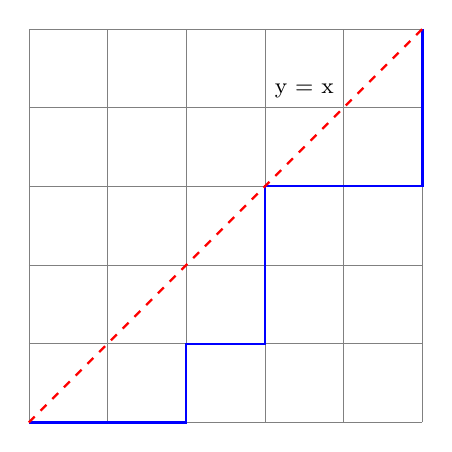
\begin{tikzpicture}
        % Draw the grid
        \draw[step=1cm,gray,very thin] (0,0) grid (5,5);

        % Draw the Dyck path
        \draw[thick,blue]
            (0,0)
            -- ++(1,0)
            -- ++(1,0)
            -- ++(0,1)
            -- ++(1,0)
            -- ++(0,1)
            -- ++(0,1)
            -- ++(1,0)
            -- ++(1,0)
            -- ++(0,1)
            -- ++(0,1);

        \draw[thick, red, dashed] (0,0) -- (5,5);
        \node[above, black] at (3.5,4) {\footnotesize y = x};

    \end{tikzpicture}
\end{document}